\documentclass[crop,tikz]{standalone}
\usetikzlibrary{backgrounds}
\colorlet{blue}{cyan}
\tikzset{
  inverted/.style = {
    every path/.style = {draw=white,text=white},
    background rectangle/.style={fill},
    show background rectangle
  }
}

\usepackage{amsmath}
\newcommand{\F}{\vec{F}}
\tikzset{>=latex}
\usetikzlibrary{patterns,decorations.pathmorphing}

\begin{document}
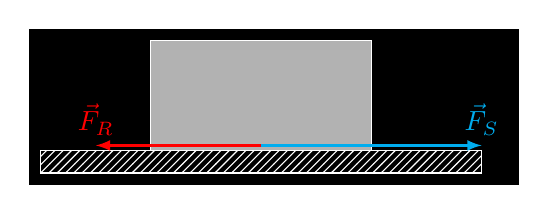
\begin{tikzpicture}[inverted,scale=1.4]
  \pattern[pattern=north east lines,pattern color=white] (-1,0)--++(0,-0.2)--++(4,0)--++(0,0.2)--cycle;
  \draw (-1,0) -- ++(4,0);
  \draw[fill=gray!60] (0,0) rectangle (2,1);
  \draw[->,thick,blue] (1,0.05) -- ++(2,0) node[above] {$\F_S$};
  \draw[->,thick,red] (1,0.05) -- ++(-1.5,0) node[above] {$\F_R$};
\end{tikzpicture}
\end{document}
